\documentclass[12pt]{beamer}

\usetheme{Oxygen}
\usepackage{thumbpdf}
\usepackage{wasysym}
\usepackage{ucs}
\usepackage[utf8]{inputenc}
\usepackage{pgf,pgfarrows,pgfnodes,pgfautomata,pgfheaps,pgfshade}
\usepackage{verbatim}




\title{EE1390}
\subtitle{Matrix Analysis Project}
\author{Govind Balaji S(cs18btech11015) \\ Madugula Sai Mehar(ee18btech11029) \\ Gugulothu Yashwanth Naik(ee18btech11017)}
%\date{February 14th, 2019}

\begin{document}

\frame{\titlepage}

\section*{}
\begin{frame}
  \frametitle{Outline}
  \tableofcontents[section=1,hidesubsections]
\end{frame}

\AtBeginSection[]
{
  \frame<handout:0>
  {
    \frametitle{Outline}
    \tableofcontents[currentsection,hideallsubsections]
  }
}

\AtBeginSubsection[]
{
  \frame<handout:0>
  {
    \frametitle{Outline}
    \tableofcontents[sectionstyle=show/hide,subsectionstyle=show/shaded/hide]
  }
}

\newcommand<>{\highlighton}[1]{%
  \alt#2{\structure{#1}}{{#1}}
}
\newcommand\numberthis{\addtocounter{equation}{1}\tag{\theequation}}

\newcommand{\icon}[1]{\pgfimage[height=1em]{#1}}



%%%%%%%%%%%%%%%%%%%%%%%%%%%%%%%%%%%%%%%%%
%%%%%%%%%% Content starts here %%%%%%%%%%
%%%%%%%%%%%%%%%%%%%%%%%%%%%%%%%%%%%%%%%%%



\section{Geometry Problem}

\begin{frame}
  \frametitle{Geometry Problem}
  \framesubtitle{Q.No 55 from JEE Advanced 2013 Paper 2}
  \begin{block}{Problem Statement}
  \begin{itemize}
    \item Let $PQ$ be a focal chord of the parabola $y^2 = 4ax$. The tangents to the parabola at $P$ and $Q$ meet at a point lying on the line $y = 2x+a, a>0$.
    \item Length of chord $PQ$ is :
  \end{itemize}
  \end{block}

  \begin{block}{Options}
  \begin{itemize}
    \item 7a \item 5a \item 2a \item 3a
  \end{itemize}
  \end{block}
\end{frame}

\section{Matrix Transformation}
\begin{frame}
  \frametitle{Matrix Transformation}

  \begin{block}{Equation of a general conic}
    \begin{center}
        $X^TVX + 2u^TX + F = 0$
    \end{center}
  \end{block}
    \begin{block}{Observe that the given parabola can be represented as:}
    \begin{center}
       $ x^T \left( {\begin{array}{cc} 0 & 0 \\ 0 & 1 \\ \end{array}} \right) x + 2 \left({\begin{array}{cc}-2a &  0\end{array}}\right)x = 0$
    \end{center}

    \end{block}  
    \begin{block}{and the given line can be represented as}
    \begin{center}$\left( \begin{array}{cc} 2 &-1\end{array}\right)x + a = 0$\end{center}
    \end{block}  
    \end{frame}
    \begin{frame}{Matrix Transformation}
        Thus the question can be re formulated as
        \begin{block}{Question}
        Let $PQ$ be a focal chord of the parabola $ x^T \left( {\begin{array}{cc} 0 & 0 \\ 0 & 1 \\ \end{array}} \right) x + 2 \left({\begin{array}{cc}-2a &  0\end{array}}\right)x = 0$. The tangents at the parabola at $P$ and $Q$ meet at point lying on the line $\left( \begin{array}{cc} 2 &-1\end{array}\right)x + a = 0, a>0$. Length of the chord $PQ$ is : 
        \end{block}
    \end{frame}
\section{Solution}
    \begin{frame}{Finding the intersection point of tangents}
    Since points P and Q lie on the parabola, \\
    \begin{equation}
        P^T \left( {\begin{array}{cc} 0 & 0 \\ 0 & 1 \\ \end{array}} \right) P + 2 \left({\begin{array}{cc}-2a &  0\end{array}}\right)P = 0  \end{equation} 
        \begin{equation}
        Q^T \left( {\begin{array}{cc} 0 & 0 \\ 0 & 1 \\ \end{array}} \right) Q + 2 \left({\begin{array}{cc}-2a &  0\end{array}}\right)Q = 0
        \end{equation}
    \end{frame}
    \begin{frame}{Finding the intersection point of tangents}
    \begin{block}{General tangent equation at p on a conic}
        \begin{center}
            $(p^TV + u^T)x + p^Tu + F= 0$
        \end{center}
    \end{block}
    Here the equations of tangents at P and Q respectively are: \\
    \begin{equation}
        \left[ P^T \left( {\begin{array}{cc} 0 & 0 \\ 0 & 1 \\ \end{array}} \right) + \left({\begin{array}{cc}-2a &  0\end{array}}\right) \right]x + P^T \left({\begin{array}{c}-2a \\  0\end{array}}\right) = 0
    \end{equation}
    \begin{equation}
        \left[ Q^T \left( {\begin{array}{cc} 0 & 0 \\ 0 & 1 \\ \end{array}} \right) + \left({\begin{array}{cc}-2a &  0\end{array}}\right) \right]x + Q^T \left({\begin{array}{c}-2a \\  0\end{array}}\right) = 0
    \end{equation}
    \end{frame}
    \begin{frame}{Finding the intersection point of tangents}
    Since PQ is a focal chord, the line joining them passes through the focus. \\
    ie. \begin{align*}
        \left({\begin{array}{c}a \\  0\end{array}}\right) &= P + \lambda (Q-P)  \\
        \left({\begin{array}{c}a \\  0\end{array}}\right) &= P(1-\lambda) + \lambda Q \numberthis
        \end{align*}
    \end{frame}
    \begin{frame}{Finding the intersection point of tangents}
    Multiply (3) with $1-\lambda$ and (4) with $ \lambda$ and add, \\
    \begin{align*}
    \left((1-\lambda)P^T+\lambda Q^T \right)\left( {\begin{array}{cc} 0 & 0 \\ 0 & 1 \\ \end{array}} \right) &+ (1-\lambda+\lambda)\left({\begin{array}{cc}-2a &  0\end{array}}\right)x \\ &+ \left( (1-\lambda)P^T + \lambda Q^T)\right)\left({\begin{array}{c}-2a \\  0\end{array}}\right) \\ &= 0 \\
    \end{align*}
    \end{frame}
    \begin{frame}{Finding the intersection point of tangents}
    Using equation (5),
    \begin{align*}
        \Rightarrow \left({\begin{array}{cc}a &  0\end{array}}\right) \left( {\begin{array}{cc} 0 & 0 \\ 0 & 1 \\ \end{array}} \right) + \left({\begin{array}{cc}-2a &  0\end{array}}\right)x + \left({\begin{array}{cc}a &  0\end{array}}\right) \left({\begin{array}{c}-2a \\  0\end{array}}\right) = 0
    \end{align*}
    On simplification this gives, 
    \begin{align*}
        \left({\begin{array}{cc}-2a &  0\end{array}}\right)x &= 2a^2 \\
        \left({\begin{array}{cc}1 &  0\end{array}}\right)x &= -a \numberthis
    \end{align*}
     \end{frame}
    \begin{frame}{Finding the intersection point of tangents}
    Also, given that this point lies on
        \begin{align*}
    \left( \begin{array}{cc} 2 &-1\end{array}\right)x &= -a \\
    \Rightarrow \left( \begin{array}{cc} 1 & 0 \\ 2 & -1 \end{array} \right) x &= \left( \begin{array}{c}-a \\ -a \end{array} \right) \\
    \Rightarrow  x &= \left( \begin{array}{c}-a \\ -a \end{array} \right) \numberthis
        \end{align*}
    \end{frame}
\begin{frame}{Finding $P-Q$}
Substitute (7) in (3),
    \begin{align*}
        \left[ P^T \left( {\begin{array}{cc} 0 & 0 \\ 0 & 1 \\ \end{array}} \right) + \left({\begin{array}{cc}-2a &  0\end{array}}\right) \right] \left( \begin{array}{c}-a \\ -a \end{array} \right) + P^T \left({\begin{array}{c}-2a \\  0\end{array}}\right) &= 0 \\
        P^T \left( {\begin{array}{cc} 0 & 0 \\ 0 & 1 \\ \end{array}} \right)\left( \begin{array}{c}-a \\ -a \end{array} \right) + \left({\begin{array}{cc}-2a &  0\end{array}}\right)\left( \begin{array}{c}-a \\ -a \end{array} \right) + P^T \left({\begin{array}{c}-2a \\  0\end{array}}\right) &= 0
    \end{align*}
    On Simplifying and taking transpose on both sides,
    \begin{align*}
        \left({\begin{array}{cc}2 &  1\end{array}}\right)P &=2a \numberthis
    \end{align*}
    Similarly on substituting (7) in (4),
    \begin{align*}
        \left({\begin{array}{cc}2 &  1\end{array}}\right)Q &=2a \numberthis
    \end{align*}
    \end{frame}
\begin{frame}{Finding $P-Q$}
Subtract (9) from (8), 
\begin{equation}
    \left({\begin{array}{cc}2 &  1\end{array}}\right)(P-Q) &=0 
\end{equation}
Observe that $ \left({\begin{array}{cc}2 &  1\end{array}}\right)\left({\begin{array}{c} 1 \\  -2\end{array}}\right)  &=0  $
\begin{block}{Note}\begin{center}
$n^Ta = n^Tb = 0 \Rightarrow a= kb $ \end{center}
\end{block}
\begin{equation}
    \Rightarrow P-Q = k \left({\begin{array}{c} 1 \\  -2\end{array}}\right)
\end{equation}
\end{frame}
\begin{frame}{Finding $P-Q$}
Thus put $P = Q + \left({\begin{array}{c} k\\  -2k\end{array}}\right)$ in (1)
\begin{align*}
    \left(Q + \left({\begin{array}{c} k\\  -2k\end{array}}\right)\right)^T &\left( {\begin{array}{cc} 0 & 0 \\ 0 & 1 \\ \end{array}} \right)  \left(Q + \left({\begin{array}{c} k\\  -2k\end{array}}\right)\right) \\ &+ 2 \left({\begin{array}{cc}-2a &  0\end{array}}\right)\left(Q + \left({\begin{array}{c} k\\  -2k\end{array}}\right)\right) = 0 
\end{align*}
\end{frame}
\begin{frame}{Finding $P-Q$}
On simplifying,
\begin{align*}
    Q^T\left( {\begin{array}{cc} 0 & 0 \\ 0 & 1 \\ \end{array}} \right) Q &+ Q^T \left({\begin{array}{c} 0\\  -2k\end{array}}\right) + \left({\begin{array}{cc}0 &  -2k\end{array}}\right)Q + 4k^2 \\ &+ 2 \left({\begin{array}{cc}-2a &  0\end{array}}\right)Q -4ak &= 0
\end{align*}
Further simplification using (2) gives,
\begin{align*}
    \left({\begin{array}{cc}0 &  1\end{array}}\right)Q = k-a \numberthis
\end{align*}
\end{frame}
\begin{frame}{Finding $P-Q$}
From (9) and (12),
\begin{align*}
    \left( \begin{array}{cc} 2 & 1 \\ 0 & 1 \end{array} \right) Q &= \left( \begin{array}{c}k-a \\ 2a \end{array} \right) \\
    \Rightarrow  Q &= \left( \begin{array}{c}\frac{3a-k}{2} \\ k-a \end{array} \right) \numberthis
\end{align*}
\end{frame}
\begin{frame}{Finding $P-Q$}
Substitute (13) in (2) with x = Q, \\
\begin{align*}
    \left[ \left({\begin{array}{cc}\frac{3a-k}{2}  & k-a\end{array}}\right)\left( {\begin{array}{cc} 0 & 0 \\ 0 & 1 \\ \end{array}} \right) + \left({\begin{array}{cc}-2a &  0\end{array}}\right) \right]\left( \begin{array}{c}\frac{3a-k}{2} \\ k-a \end{array} \right) \\ + \left({\begin{array}{cc}\frac{3a-k}{2} &  k-a\end{array}}\right) \left({\begin{array}{c}-2a \\  0\end{array}}\right) &= 0
\end{align*}
\end{frame}
\begin{frame}{Finding $P-Q$}
On simplification finally yields, \\
\begin{align*}
     k^2 &= 5a^2 \\ \Rightarrow k &= \pm \sqrt{5} a \\
     P-Q &= \pm \sqrt{5}a \left({\begin{array}{c}1 \\  -2\end{array}}\right) \\
     \Rightarrow ||P-Q|| &= 5a
\end{align*}
\begin{block}{Answer}
\begin{center}
Thus the length $ PQ = 5a $ 
\end{center}
\end{block}
\end{frame}

\section{Python verification}
\begin{frame}{Python verification}
The points and lines given in the question and those obtained in solution are plotted using pyplot library. The distance PQ is verified as $5a$
\end{frame}
\begin{frame}{Python verification}
\begin{block}{Plot}
\begin{center}
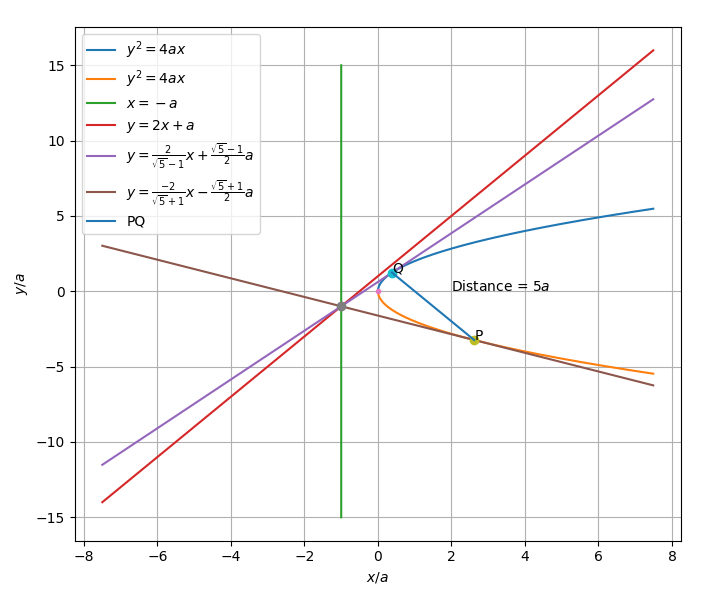
\includegraphics[scale=0.3]{figs/pyplot.png}
\end{center}
\end{block}

\end{frame}

\end{document}
